% Options for packages loaded elsewhere
\PassOptionsToPackage{unicode}{hyperref}
\PassOptionsToPackage{hyphens}{url}
\PassOptionsToPackage{dvipsnames,svgnames,x11names}{xcolor}
%
\documentclass[
  12pt,
]{article}
\usepackage{amsmath,amssymb}
\usepackage{iftex}
\ifPDFTeX
  \usepackage[T1]{fontenc}
  \usepackage[utf8]{inputenc}
  \usepackage{textcomp} % provide euro and other symbols
\else % if luatex or xetex
  \usepackage{unicode-math} % this also loads fontspec
  \defaultfontfeatures{Scale=MatchLowercase}
  \defaultfontfeatures[\rmfamily]{Ligatures=TeX,Scale=1}
\fi
\usepackage{lmodern}
\ifPDFTeX\else
  % xetex/luatex font selection
\fi
% Use upquote if available, for straight quotes in verbatim environments
\IfFileExists{upquote.sty}{\usepackage{upquote}}{}
\IfFileExists{microtype.sty}{% use microtype if available
  \usepackage[]{microtype}
  \UseMicrotypeSet[protrusion]{basicmath} % disable protrusion for tt fonts
}{}
\makeatletter
\@ifundefined{KOMAClassName}{% if non-KOMA class
  \IfFileExists{parskip.sty}{%
    \usepackage{parskip}
  }{% else
    \setlength{\parindent}{0pt}
    \setlength{\parskip}{6pt plus 2pt minus 1pt}}
}{% if KOMA class
  \KOMAoptions{parskip=half}}
\makeatother
\usepackage{xcolor}
\usepackage[margin=1in]{geometry}
\usepackage{color}
\usepackage{fancyvrb}
\newcommand{\VerbBar}{|}
\newcommand{\VERB}{\Verb[commandchars=\\\{\}]}
\DefineVerbatimEnvironment{Highlighting}{Verbatim}{commandchars=\\\{\}}
% Add ',fontsize=\small' for more characters per line
\usepackage{framed}
\definecolor{shadecolor}{RGB}{248,248,248}
\newenvironment{Shaded}{\begin{snugshade}}{\end{snugshade}}
\newcommand{\AlertTok}[1]{\textcolor[rgb]{0.94,0.16,0.16}{#1}}
\newcommand{\AnnotationTok}[1]{\textcolor[rgb]{0.56,0.35,0.01}{\textbf{\textit{#1}}}}
\newcommand{\AttributeTok}[1]{\textcolor[rgb]{0.13,0.29,0.53}{#1}}
\newcommand{\BaseNTok}[1]{\textcolor[rgb]{0.00,0.00,0.81}{#1}}
\newcommand{\BuiltInTok}[1]{#1}
\newcommand{\CharTok}[1]{\textcolor[rgb]{0.31,0.60,0.02}{#1}}
\newcommand{\CommentTok}[1]{\textcolor[rgb]{0.56,0.35,0.01}{\textit{#1}}}
\newcommand{\CommentVarTok}[1]{\textcolor[rgb]{0.56,0.35,0.01}{\textbf{\textit{#1}}}}
\newcommand{\ConstantTok}[1]{\textcolor[rgb]{0.56,0.35,0.01}{#1}}
\newcommand{\ControlFlowTok}[1]{\textcolor[rgb]{0.13,0.29,0.53}{\textbf{#1}}}
\newcommand{\DataTypeTok}[1]{\textcolor[rgb]{0.13,0.29,0.53}{#1}}
\newcommand{\DecValTok}[1]{\textcolor[rgb]{0.00,0.00,0.81}{#1}}
\newcommand{\DocumentationTok}[1]{\textcolor[rgb]{0.56,0.35,0.01}{\textbf{\textit{#1}}}}
\newcommand{\ErrorTok}[1]{\textcolor[rgb]{0.64,0.00,0.00}{\textbf{#1}}}
\newcommand{\ExtensionTok}[1]{#1}
\newcommand{\FloatTok}[1]{\textcolor[rgb]{0.00,0.00,0.81}{#1}}
\newcommand{\FunctionTok}[1]{\textcolor[rgb]{0.13,0.29,0.53}{\textbf{#1}}}
\newcommand{\ImportTok}[1]{#1}
\newcommand{\InformationTok}[1]{\textcolor[rgb]{0.56,0.35,0.01}{\textbf{\textit{#1}}}}
\newcommand{\KeywordTok}[1]{\textcolor[rgb]{0.13,0.29,0.53}{\textbf{#1}}}
\newcommand{\NormalTok}[1]{#1}
\newcommand{\OperatorTok}[1]{\textcolor[rgb]{0.81,0.36,0.00}{\textbf{#1}}}
\newcommand{\OtherTok}[1]{\textcolor[rgb]{0.56,0.35,0.01}{#1}}
\newcommand{\PreprocessorTok}[1]{\textcolor[rgb]{0.56,0.35,0.01}{\textit{#1}}}
\newcommand{\RegionMarkerTok}[1]{#1}
\newcommand{\SpecialCharTok}[1]{\textcolor[rgb]{0.81,0.36,0.00}{\textbf{#1}}}
\newcommand{\SpecialStringTok}[1]{\textcolor[rgb]{0.31,0.60,0.02}{#1}}
\newcommand{\StringTok}[1]{\textcolor[rgb]{0.31,0.60,0.02}{#1}}
\newcommand{\VariableTok}[1]{\textcolor[rgb]{0.00,0.00,0.00}{#1}}
\newcommand{\VerbatimStringTok}[1]{\textcolor[rgb]{0.31,0.60,0.02}{#1}}
\newcommand{\WarningTok}[1]{\textcolor[rgb]{0.56,0.35,0.01}{\textbf{\textit{#1}}}}
\usepackage{longtable,booktabs,array}
\usepackage{calc} % for calculating minipage widths
% Correct order of tables after \paragraph or \subparagraph
\usepackage{etoolbox}
\makeatletter
\patchcmd\longtable{\par}{\if@noskipsec\mbox{}\fi\par}{}{}
\makeatother
% Allow footnotes in longtable head/foot
\IfFileExists{footnotehyper.sty}{\usepackage{footnotehyper}}{\usepackage{footnote}}
\makesavenoteenv{longtable}
\usepackage{graphicx}
\makeatletter
\def\maxwidth{\ifdim\Gin@nat@width>\linewidth\linewidth\else\Gin@nat@width\fi}
\def\maxheight{\ifdim\Gin@nat@height>\textheight\textheight\else\Gin@nat@height\fi}
\makeatother
% Scale images if necessary, so that they will not overflow the page
% margins by default, and it is still possible to overwrite the defaults
% using explicit options in \includegraphics[width, height, ...]{}
\setkeys{Gin}{width=\maxwidth,height=\maxheight,keepaspectratio}
% Set default figure placement to htbp
\makeatletter
\def\fps@figure{htbp}
\makeatother
\setlength{\emergencystretch}{3em} % prevent overfull lines
\providecommand{\tightlist}{%
  \setlength{\itemsep}{0pt}\setlength{\parskip}{0pt}}
\setcounter{secnumdepth}{-\maxdimen} % remove section numbering
% definitions for citeproc citations
\NewDocumentCommand\citeproctext{}{}
\NewDocumentCommand\citeproc{mm}{%
  \begingroup\def\citeproctext{#2}\cite{#1}\endgroup}
\makeatletter
 % allow citations to break across lines
 \let\@cite@ofmt\@firstofone
 % avoid brackets around text for \cite:
 \def\@biblabel#1{}
 \def\@cite#1#2{{#1\if@tempswa , #2\fi}}
\makeatother
\newlength{\cslhangindent}
\setlength{\cslhangindent}{1.5em}
\newlength{\csllabelwidth}
\setlength{\csllabelwidth}{3em}
\newenvironment{CSLReferences}[2] % #1 hanging-indent, #2 entry-spacing
 {\begin{list}{}{%
  \setlength{\itemindent}{0pt}
  \setlength{\leftmargin}{0pt}
  \setlength{\parsep}{0pt}
  % turn on hanging indent if param 1 is 1
  \ifodd #1
   \setlength{\leftmargin}{\cslhangindent}
   \setlength{\itemindent}{-1\cslhangindent}
  \fi
  % set entry spacing
  \setlength{\itemsep}{#2\baselineskip}}}
 {\end{list}}
\usepackage{calc}
\newcommand{\CSLBlock}[1]{\hfill\break\parbox[t]{\linewidth}{\strut\ignorespaces#1\strut}}
\newcommand{\CSLLeftMargin}[1]{\parbox[t]{\csllabelwidth}{\strut#1\strut}}
\newcommand{\CSLRightInline}[1]{\parbox[t]{\linewidth - \csllabelwidth}{\strut#1\strut}}
\newcommand{\CSLIndent}[1]{\hspace{\cslhangindent}#1}
\usepackage{graphicx}
\ifLuaTeX
  \usepackage{selnolig}  % disable illegal ligatures
\fi
\usepackage{bookmark}
\IfFileExists{xurl.sty}{\usepackage{xurl}}{} % add URL line breaks if available
\urlstyle{same}
\hypersetup{
  pdftitle={Reproduceable Research},
  pdfauthor={Ina Krapp},
  colorlinks=true,
  linkcolor={Maroon},
  filecolor={Maroon},
  citecolor={Blue},
  urlcolor={blue},
  pdfcreator={LaTeX via pandoc}}

\title{Reproduceable Research}
\author{Ina Krapp}
\date{2025-04-07}

\begin{document}
\maketitle

\subsection{This is an example research
document:}\label{this-is-an-example-research-document}

We will load some data, perform an analysis, visualize the results and
compile it all into a nice document.

Markdown is a simpler language for creating text documents than Latex.
For example, to let text appear in a new line, leave a line blank:

As you can see, this text appears in a new line. To make a list, simply
number your points: For our analysis, we will:

\begin{enumerate}
\def\labelenumi{\arabic{enumi}.}
\item
  Get some data.
\item
  Clean it up.
\item
  Create some summary statistics
\item
  Run a regression
\item
  Visualize the result
\end{enumerate}

Or create a list with dots. We will use R Markdown to create PDF
documents today, but R Markdown can generate a wide range of formats,
including:

\begin{itemize}
\item
  HTML Websites
\item
  Word Documents
\item
  PowerPoint Presentations.
\end{itemize}

It also has a Visual editor: If you have an R Markdown file open, click
on `Visual' in the upper left area to open it. It makes things like
adding an image or a citation easier. Below is an example image I
inserted using the visual editor:

\begin{figure}
\centering
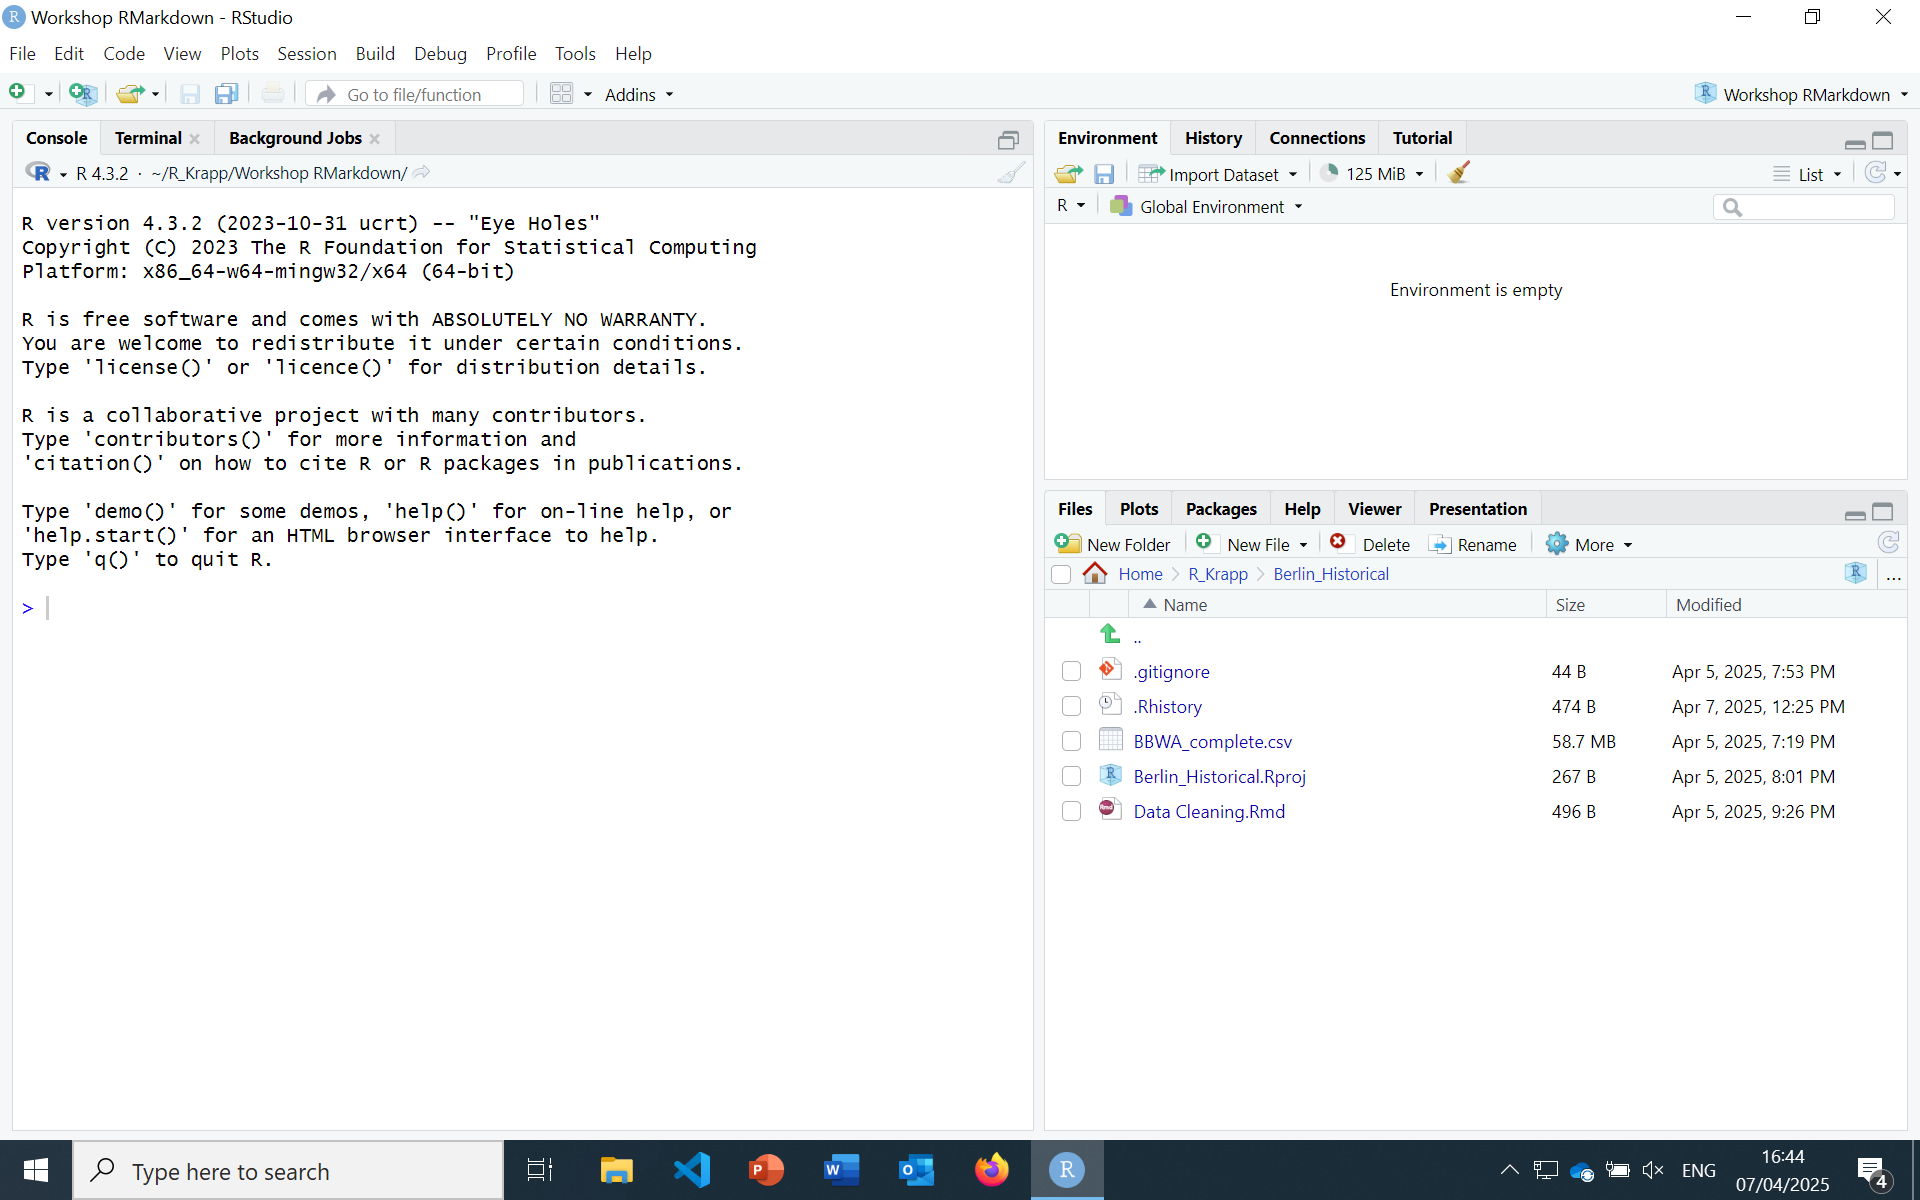
\includegraphics{RStudio.png}
\caption{This is an example image.}
\end{figure}

This file can also include Latex code you'd like to use. For equations,
Latex is typically used: \(y = x\beta + \epsilon\).

One can create sub-headers by using hash signs: One hash is used for the
header of the document, two for the headers of chapters, three for
sub-headers of the chapters and so on. (We already have a title field in
the YAML header above, so we typically only use two or more hashes).

\subsubsection{This is an example
sub-header.}\label{this-is-an-example-sub-header.}

A major strength of R Markdown is the combination of text and code: The
text below alternates with R-Code (so-called `chunks'). Each chunk can
be run individually, but for creating a document, they are run in order.

Instead of copy-pasting figures or tables into the document, you can
directly create them within R in R Markdown. Or another programming
language:

\begin{Shaded}
\begin{Highlighting}[]
\BuiltInTok{print}\NormalTok{(}\StringTok{"Hello! I am python code!"}\NormalTok{)}
\end{Highlighting}
\end{Shaded}

\begin{verbatim}
## Hello! I am python code!
\end{verbatim}

Supported languages include also Julia, C++ and SQL.

\subsection{Obtain the data}\label{obtain-the-data}

We will get some data on when the cherry blossoms bloom in Japan:
\href{https://github.com/tacookson/data/tree/master/sakura-flowering}{Link
to the cherry blossom data}.

The data is taken from Aono and Saito (2010). One can also cite with
parenthesis by using square brackets: (Aono and Saito 2010). The visual
editor automatically adds square brackets unless the `In-text' option is
ticked.

A bibliography is automatically added at the end of the document.

Code can be embedded like this:

\begin{Shaded}
\begin{Highlighting}[]
\CommentTok{\# Load data:}
\NormalTok{sakura\_modern }\OtherTok{\textless{}{-}} \FunctionTok{read\_csv}\NormalTok{(}\StringTok{"https://raw.githubusercontent.com/tacookson/data/master/sakura{-}flowering/sakura{-}modern.csv"}\NormalTok{)}
\end{Highlighting}
\end{Shaded}

\begin{verbatim}
## Rows: 6700 Columns: 9
## -- Column specification --------------------------------------------------------
## Delimiter: ","
## chr  (1): station_name
## dbl  (6): station_id, latitude, longitude, year, flower_doy, full_bloom_doy
## date (2): flower_date, full_bloom_date
## 
## i Use `spec()` to retrieve the full column specification for this data.
## i Specify the column types or set `show_col_types = FALSE` to quiet this message.
\end{verbatim}

\begin{Shaded}
\begin{Highlighting}[]
\NormalTok{temperatures\_modern }\OtherTok{\textless{}{-}} \FunctionTok{read\_csv}\NormalTok{(}\StringTok{"https://raw.githubusercontent.com/tacookson/data/master/sakura{-}flowering/temperatures{-}modern.csv"}\NormalTok{)}
\end{Highlighting}
\end{Shaded}

\begin{verbatim}
## Rows: 81600 Columns: 6
## -- Column specification --------------------------------------------------------
## Delimiter: ","
## chr  (2): station_name, month
## dbl  (3): station_id, year, mean_temp_c
## date (1): month_date
## 
## i Use `spec()` to retrieve the full column specification for this data.
## i Specify the column types or set `show_col_types = FALSE` to quiet this message.
\end{verbatim}

These r chunks are visible by default in the text. We also see all the
messages it generated. For scientific reports or papers, we usually do
not want that. We can turn it off using chunk options.

\subsection{Clean up the data}\label{clean-up-the-data}

The first step once we obtained the data is to clean it. The code below
combines the two datasets, removes missing values and a few columns we
will not use, and aggregates temperature to yearly averages.

The chunk option `echo' controls if the code is displayed. It is set to
false in this chunk, so the code will not show in the PDF document.

There are various other chunk options to control if the code or any
output of it (text, figures, warnings\ldots) should be displayed.

This code below here has `eval = FALSE' set as chunk option. This means
it will not run for now. We will come back to it later.

While ``include = FALSE'' means we can run code without displaying it in
the PDF, it also means we currently don't see any results. There are
other ways to modify the code. A few common ones:

include = FALSE prevents code and results from appearing in the pdf
file. R Markdown still runs the code in the chunk, and the results can
be used by other chunks.

echo = FALSE prevents code, but not the results from appearing in the
pdf file. This is a useful way to embed figures.

message = FALSE prevents messages that are generated by code from
appearing in the pdf file.

warning = FALSE prevents warnings that are generated by code from
appearing in the pdf file.

\subsection{Create summary statistics:}\label{create-summary-statistics}

Tables can be nicely displayed in R Markdown using the kable package.
Below, a summary table is created and then displayed using `kable'.
kable is highly customizeable, but its defaults usually do not look bad,
either.

\begin{longtable}[]{@{}
  >{\centering\arraybackslash}p{(\columnwidth - 6\tabcolsep) * \real{0.1591}}
  >{\centering\arraybackslash}p{(\columnwidth - 6\tabcolsep) * \real{0.2121}}
  >{\centering\arraybackslash}p{(\columnwidth - 6\tabcolsep) * \real{0.2879}}
  >{\centering\arraybackslash}p{(\columnwidth - 6\tabcolsep) * \real{0.3409}}@{}}
\caption{Summary statistics of the cherry blossom data.}\tabularnewline
\toprule\noalign{}
\begin{minipage}[b]{\linewidth}\centering
Average Temperature
\end{minipage} & \begin{minipage}[b]{\linewidth}\centering
St.~Deviation: Temperature
\end{minipage} & \begin{minipage}[b]{\linewidth}\centering
Average Day of first flowers opening
\end{minipage} & \begin{minipage}[b]{\linewidth}\centering
St.~Deviation: Day of first flowers opening
\end{minipage} \\
\midrule\noalign{}
\endfirsthead
\toprule\noalign{}
\begin{minipage}[b]{\linewidth}\centering
Average Temperature
\end{minipage} & \begin{minipage}[b]{\linewidth}\centering
St.~Deviation: Temperature
\end{minipage} & \begin{minipage}[b]{\linewidth}\centering
Average Day of first flowers opening
\end{minipage} & \begin{minipage}[b]{\linewidth}\centering
St.~Deviation: Day of first flowers opening
\end{minipage} \\
\midrule\noalign{}
\endhead
\bottomrule\noalign{}
\endlastfoot
6.623789 & 0.5935223 & 95.25429 & 23.46164 \\
\end{longtable}

We can rightfully assume that there is a correlation between the day the
first flowers open and the day most flowers are open - in warmer areas,
flowers open earlier and the tree is also in full bloom earlier. R
Markdown allows to use inline code: The correlation is 0.99127 . To
round it, we can use the round function: 0.99.

\subsection{The analysis:}\label{the-analysis}

Because of global warming, the average temperature has increased. Do the
cherry blossoms also bloom earlier now than in the past?

Yes. As we can see, the year has an impact - the bloom has been starting
earlier in recent years because of global warming.

\begin{longtable}[]{@{}ll@{}}
\caption{Regression results: Impact of the year on cherry blossom bloom
time.}\tabularnewline
\toprule\noalign{}
& Summary of the regression \\
\midrule\noalign{}
\endfirsthead
\toprule\noalign{}
& Summary of the regression \\
\midrule\noalign{}
\endhead
\bottomrule\noalign{}
\endlastfoot
Dependent Var.: & flower\_doy \\
& \\
Constant & 504.6*** (84.44) \\
year & -0.2062*** (0.0432) \\
\_\_\_\_\_\_\_\_\_\_\_\_\_\_\_ &
\_\_\_\_\_\_\_\_\_\_\_\_\_\_\_\_\_\_\_ \\
S.E.: Clustered & by: longitude-lat.. \\
Observations & 5,655 \\
R2 & 0.02509 \\
Adj. R2 & 0.02491 \\
\end{longtable}

We can display the data and the line fitted through it using ggplot.
Below, we also use fig.cap = ``\ldots{}'', it adds a caption to the
created graph.

\begin{figure}
\centering
\includegraphics{Reproduceable-Research-with-R-Markdown_files/figure-latex/unnamed-chunk-8-1.pdf}
\caption{Change in the cherry blossom bloom time since the 1950's.}
\end{figure}

As we can see, there were always places where the flowers bloomed
particularly early, sometimes even in early January (these are Japan's
southern islands, like Okinawa). However, there is a clear downward
trend: The years are getting warmer and the cherry blossoms bloom
earlier.

But wait, a few observations appear to be missing. For example, around
1970, no points exist in the first two months of the year, which likely
indicates that measurements from the southern islands are missing in
this period. Does the trend stay the same if we only include
observations of places which were observed continously through the
entire timespan?

You can find out by setting the option `eval = FALSE' in the code chunk
at the beginning to `eval = TRUE'. As you can see, including only the
stations which cover the entire timespan, the graph looks very
different. Note that all other values in the document (like the
correlation calculated above) also changed. However, the temperature
trend persisted.

Finally, if you still need Latex, you can add `keep\_tex: True' in the
YAML header. R Markdown automatically uses Latex when producing a PDF,
so you can simply look at the Latex file it already generated.

For anyone who would like to learn more about R Markdown and its
capabilities, I highly recommend the
\href{https://bookdown.org/yihui/R\%20Markdown-cookbook/}{R Markdown
cookbook}. And for anyone who wishes to go deeper (including, for
example, learning how to write entire books with R Markdown), I
recommend \href{https://bookdown.org/yihui/rmarkdown/}{R Markdown: The
Definitive Guide}

\subsection*{Bibliography}\label{bibliography}
\addcontentsline{toc}{subsection}{Bibliography}

\phantomsection\label{refs}
\begin{CSLReferences}{1}{0}
\bibitem[\citeproctext]{ref-aonoClarifyingSpringtimeTemperature2010}
Aono, Yasuyuki, and Shizuka Saito. 2010. {``Clarifying Springtime
Temperature Reconstructions of the Medieval Period by Gap-Filling the
Cherry Blossom Phenological Data Series at {Kyoto}, {Japan}.''}
\emph{International Journal of Biometeorology} 54 (2): 211--19.
\url{https://doi.org/10.1007/s00484-009-0272-x}.

\end{CSLReferences}

\end{document}
